% !TEX encoding = UTF-8 Unicode
\documentclass[conference]{IEEEtran}
\IEEEoverridecommandlockouts
% The preceding line is only needed to identify funding in the first footnote. If that is unneeded, please comment it out.
%\usepackage[dashed=false]{biblatex}
\usepackage{cite}
\usepackage{amsmath,amssymb,amsfonts}
\usepackage{algorithmic}
\usepackage{graphicx}
\usepackage{textcomp}
\usepackage{xcolor}
\usepackage{tikz}
\usepackage{multirow}
\usepackage{footnote}
\usepackage{float}
\usepackage{verbatim}

\makesavenoteenv{tabular}
\usetikzlibrary{positioning,shapes,backgrounds,arrows}
\usetikzlibrary{decorations.pathmorphing}

\renewcommand{\theenumi}{\alph{enumi}}

\def\thesubsectiondis{\arabic{subsection}.}

\def\thesubsubsectiondis{\arabic{subsection}.\arabic{subsubsection}}

\def\theparagraphdis{\arabic{subsection}.\arabic{subsubsection}.\arabic{paragraph}}

\def\BibTeX{{\rm B\kern-.05em{\sc i\kern-.025em b}\kern-.08em
    T\kern-.1667em\lower.7ex\hbox{E}\kern-.125emX}}
\begin{document}

\title{Operational efficiency prediction in thinning and clear-cutting using artificial neural networks\\
}

\author{
\IEEEauthorblockN{Hugo Ubilla, Rodrigo de la Fuente, Eduardo Acuña}
\IEEEauthorblockA{\textit{Departamento de Ingeniería Industrial} \\
\textit{Universidad de Concepción}\\
Concepción, Chile \\
hugoubilla@udec.cl, radelafu@ncsu.edu, edacuna@udec.cl}
\and
\IEEEauthorblockN{Felipe Sepulveda}
\IEEEauthorblockA{\textit{Departamento de Ingeniería Industrial} \\
\textit{Universidad de Chile}\\
Santiago, Chile \\
felisepulveda@udec.cl}
}

\maketitle

\begin{abstract} 
The forestry sector is fundamental to Chile's economic development. Clear-cutting and thinning are two paramount processes in the forestry industry. In this article, artificial neural networks are used to estimate crop yields and analyze the thinning process. A multi-layer perceptron neural network is used to obtain clear-cutting forecasts, and a self-organized map (SOM) network to examine the thinning process. Both models are executed using GPU training in TensorFlow. For forecasting, 768 neural network configurations are implemented. The one with the best performance is selected based on the mean squared error criterion. The results are compared with those obtained in linear regression, showing a MSE and $r^2$ of 2484.56 and 0.78 respectively, versus 3979.21 and 0.64 obtained in the best linear regression model. Furthermore, three SOM structures are tested with three different number of nodes, a 2-dimensional, a toroidal and a 3-dimensional lattice. The best network corresponds to a 3-dimensional structure of $9\times9\times9$ nodes. Additionally, the algorithms of k-means and silhouette coefficient are used to generate clusters. The best structure is selected by quantization error. Three clusters are obtained, and the analysis show that the attribute of slope of the land has greater influence in the thinning process. The results of both procedures ensure that both artificial neural networks are powerful tools for estimation and data analysis.
\end{abstract}

\begin{IEEEkeywords}
artifical neural network, self-organizing maps, machine learning, forecasting, clear-cutting, clear-cutting.
\end{IEEEkeywords}

\section{Introduction}

The set of forest-based enterprises comprises the entire production chain of forest resources in Chile: it integrates forestry and clear-cutting activities, wood and paper industries, as well as support providers and services. Thus, the development of forestry is fundamental in the country's economic activity. In terms of exports, the Chilean forestry sector is the third largest sector of the country after the mining and food sectors. In 2017, it represented 2.7\% of the national GDP, generated 114,000 jobs and around 5,376  USD million FOB in exports, showing a 3\% increase over the previous year. The main products exported are cellulose and wood remanufacturing (47.5\% and 13.3\% of total forest products respectively). The business structure consists mainly of two types: 1) large-scale, vertically integrated and globally competitive industries, 2) a multitude of small and medium-sized enterprises engaged primarily in the domestic forest market \cite{udec_2019}.

Chile has 13.6 million hectares of native forests and 2.4 million hectares of plantations, dominated by species of the genus Pinus and Eucalyptus. Ninety percent of industrial wood is sent to sawmills, wood panels, and the pulp and paper industry. Additionally, forest is highly productive with shorter rotation periods than in the countries of the northern hemisphere, a comparative advantage for Chile.

The growth of forestry activity has made necessary to incorporate new technologies and more efficient systems in forestry operations. The critical factor in the Chilean forestry activity has been the need to achieve greater productivity under parameters of sustainability and competitive costs. Within the forest production cycle, forest clear-cutting is one of the main costs of material supply to forest enterprises, estimated between 25\% and 30\% of the total cost of the product \cite{conrad_2018}, \cite{deli_2016}, \cite{jacovine_2005},\cite{Irigoyen_2002},\cite{largo_1996}.

In this way, companies have gradually made larger investments towards the mechanization of processes. In this sense, forest exploitation has had an extraordinary development in the last years, thanks to the incorporation of state of the art machinery that not only has increased productivity but also operational safeness. The main innovations in the field of clear-cutting are focused on the turning, trimming, cutting and extraction of trees, with the incorporation of harvesters, feller bunchers and skidders of last generation \cite{lignum_2002}, \cite{lignum_2004}.

Forest utilization activities are carried out through contractors in Chile. This system is the most common method for forest plantations owners. To meet increases in demand, reduce environmental impact, and react to increasing competition in globalized markets, Chilean companies targeted growth by introducing new technologies, while reducing their clear-cutting costs and thus increasing productivity.

Historical data indicate that world production and trade in forest products have increased in recent years. This trend is expected to continue due to increased global market share among timber-exporting countries and increased production volume \cite{Hashiramotois_2004}. Thus, the future competitiveness and sustainability of the industry will be determined by how contractors can adapt to the changing environment, which will depend on improving their operational performance \cite{vahid_2007}. Consequently, in the logging sub-sector, where competition is increasing, inefficient units are expected to exit the market. It is therefore essential for the forest industry to continuously measure and improve operational efficiency if its goal is to remain competitive, in both, local and international markets.

Measurement of the operational efficiency of logging contractors has preferably been done using non-parametric techniques such as \textit{Data Envelopment Analysis} (DEA) in \cite{obi_2017}, \cite{trzcianowska_2019} or through comparative assessment of technical and economic factors in forest clear-cutting \cite{di_fulvio_2017_benchmarking}, \cite{eriksson_2015_management}, \cite{keefe_2019_smartphone},\cite{mac_2017_harvesting}. However, the use of machine learning techniques is still relatively new in forestry literature. \textit{Machine Learning} (ML) comprises the set of tools employed to teach a system how it can learn from data. Within ML, there are two main areas: supervised learning and unsupervised learning. The first one trains an algorithm to be able to predict a signal, while the second one is used to find clusters and patterns in the data.

In agro-forestry problems, different ML tools, such as, TensorFlow, Theano, Matlab, and Caffee have been applied. \cite{image_recognition1450} use TensorFlow to assess crop diseases by image recognition through a \textit{Convolutional Neural Network} (CNN). In \cite{farmland_scene}, cropland classification is performed using CNN through images. In \cite{deep_learning_class123}, TensorFlow is used in recognition of land cover and crop types using satellite imagery. This study also uses SOMs to correct distortion in images. In a related field, images of the melon leaves have been used to classify melons as good or bad using a CNN \cite{bitter_melon_villa}, employing Keras and Tensorflow to compare the generated models. In \cite{cloud_based_jain} images are used to classify plant diseases and determine whether crops are healthy. The CNN and SVM classification algorithms are compared by selecting the one with the lowest misclassification rate, by means of the Theano library. Khan et al. \cite{CCDF_automatic_khan} implement an automatic classification and segmentation system of fruit crop diseases using the correlation coefficient and CNN's. In \cite{weed_detection_ferreira} CNNs are used for the detection and classification of weeds in soybean crop images. In \cite{CCDF_automatic_khan} and \cite{weed_detection_ferreira} the Caffee library is used for miscellaneous forestry applications.

In a study published by Bhering et al. \cite{application_of_bhering}, the volume of eucalyptus wood is predicted using ANN and compared with regression models. The neuronal network used has 3 hidden layers, the first with 1 to 10 neurons, the second with 1 to 20 and the third with 1 to 8 neurons. They use 1000 epochs and 3 different activation functions. It was obtained an $r^2$ of 0.9603 and 0.9836 opposite to 0.9426 and 0.9616 of the multiple regression for data of between 3 and 6 years respectively. Neural networks have also been applied to predict mortality and survival of Atlantic Forest trees in Brazil \cite{artificial_neural_rocha}, \cite{Estimation_of_Reis}.

Similar ANN-based studies are used to predict corn and soybean yield. In \cite{artificial_neural_kaul}, an ANN is compared with linear regression. ANN obtained better results than linear regression models. The $r^2$ in corn crop yield was 0.77 for the ANN, while a 0.42 for linear regression. An $r^2$ of 0.81 was obtained for the yield of soybean crops, and 0.46 for linear regression. Conversely, in \cite{artificial_neural_gabriela}, a ANN was trained to predict certain type of pigmentation on the leaves. An $r^2$ of 0.537 is obtained in the best case. It shows no improvement concerning regression models. 

Some researches seek to predict the yield of wheat crops. Forecasts have been made in \cite{application_of_panda} through 4 types of spectral indices, obtaining an $r^2$ of more than 97\% for the best model. Authors Shastry et al. \cite{a_parameter_shastry} use rainfall, crop biomass, soil evaporation and transpiration, water extractable from the soil, and fertilizer percentage to make forecasts. The best result was obtained with two hidden layers, where the first one had 50 neurons, while the second one only 20. In \cite{crop_yield_guo}, historical information associated with planting area, rainfall and temperature are used. It is concluded that spatial neural networks deliver better prediction than autoregressive models of neural networks. In another study, wheat yield is predicted in a 22-hectare field using satellite imagery and online data using SOMs based on supervised learning \cite{wheat_yield_pantazi}. 

Rice crop yields have also been studied. In \cite{rice_crop_gandhi}, the yield is predicted and the factors affecting its production are investigated using ANN. In \cite{predicting_rice_hossain}, an ANN-based model is created to predict climate parameters and then the rice yield is estimated using \textit{Support Vector Regression} (SVR), which uses the ANN result as input. In \cite{evaluation_of_bappa} they relied on climate parameters to make predictions. \textit{Stepwise multiple linear regression} (SMLR), ANN, ANN combined with PCA, and penalized regression models are used. An $r^2$ between 0.22 and 0.98 is reached in ANN models for the testing sets.

Applications of SOMs have been found in the area of agriculture. SOMs are used in a study published in 2017 \cite{devoloping_herbicide_sachini}. The study seeks to improve the resistance of rice to herbicides in different rice varieties and herbicide concentrations. ANNs are used to visualize agro-morphological characteristics of rice varieties within the process. In \cite{the_self_organazing_mokarram}, the attributes related to wheat yield through SOM were classified using more than 11 thousand data samples with 13 attributes. Authors Venkatesh and Thangaraj \cite{self_organazing_venkatesh} investigated soil characteristics to determine suitable crop types for a region. SOM is used to analyze soil data spread over a large geographical area and to identify suitable crops for each particular soil. In \cite{artificial_neural_Waidyarathne}, states of plant disease are classified using visual symptoms. SOM is used to classify the disease based on the 3 symptoms and then clustered by k-means to find 3 different disease states. A summary of the articles from ANNs and SOMs can be found in the Table~\ref{table01} and Table~\ref{table02} respectively. 

The use of SOMs has been rarely used in forestry studies, some of its applications have been in the determination of organic C content in riparian forest areas through terrestrial measurements and satellite data, which served as input data to carry out the process of learning and training of a neural network, resulting in a spatial pattern of organic C distribution \cite{suchenwirth2014large}. Search for stand scale risk patterns for diseases and pests \cite{park2013hazard}, to predict new invasive species and prioritise species for Pest risk analyses \cite{eschen2014likelihood}. Besides, it was used SOMs in the classification of tree species in hyperspectral image \cite{malathy2016classification}.

This research is based on \textit{Artificial Neural Networks} (ANNs) of \textit{Multilayer Perceptron} type (MLP) and \textit{Self-Organizing Maps} (SOMs). The MLP is a computational model of supervised learning based on the biological neuronal processes that occur in our brains. SOMs are a type of unsupervised ML model that allows multidimensional data analysis and visualization. They were first defined by Kohonen in \cite{kohonen1982self},\cite{kohonen19822}. Generally, data visualization is done through 2 dimensions. However, other structures have been applied in the literature. This algorithm searches for and gathers similar patterns where nearby vectors are closer together within the map \cite{kohonen1995springer}.

\begin{table}[!ht]
\renewcommand{\arraystretch}{1.3}
\caption{Overview of articles on MLP}
\label{table01}
\centering
\begin{minipage}{1\linewidth} 
\resizebox{\textwidth}{!}{%

\begin{tabular}{c || c || c || c}
\hline
\bfseries Article & \bfseries Layers\footnote{The number of nodes per layer is in parentheses} & \bfseries Nº Models &  \bfseries Software \\
\hline\hline

\cite{application_of_bhering} 	& 1 Input (2) / 3 Mid (1-10,1-20,1-8) / 1 Output (1) & 43,200 & Matlab \\

\cite{artificial_neural_rocha} 	& 1 Input (5-12) / 1 Mid / 1 Output (1)  	& 1,200 & Statistica 13	\\

\cite{Estimation_of_Reis}    	& 1 Input (7-8) / 1 Mid / 1 Output (1)  	& - & Statistica 13	\\

\cite{artificial_neural_kaul}   	& 1 Input (1-20) / 1 Mid (4-7) / 1 Output (1) 	& Over 120 & 	\\

\cite{artificial_neural_gabriela}  & 1 Input / 1-3 Mid (1 - 500) / 1 Output  	& 1500 & SNNS \\
\cite{application_of_panda}  	& 1 Input (2) / 1 Mid (1) / 1 Output (1) 	& - & NW Pro II Plus \\
\cite{a_parameter_shastry}   	& 1 Input / (1 - 2) Mid (20 - 100) / 1 Output  	& - & Matlab R2013A\\
\cite{crop_yield_guo}  		& 1 Input / 1 Mid (100 - 200) / 1 Output  	& - & - \\
\cite{wheat_yield_pantazi}  	& -	& -	& Matlab \\
\cite{rice_crop_gandhi}  		& 1 Input (6) / 1 Mid (4) / 1 Output (3)	& - & WEKA	\\
\cite{predicting_rice_hossain}  	& 1 Input (9) / - Mid / 1 Output (21)	& - & WEKA	\\
\cite{evaluation_of_bappa} 	& 1 Input / 1 Mid / 1 Output 	& - 	& R \\

\hline
\end{tabular}
}
\end{minipage}
\end{table}

\begin{table}[!ht]
\renewcommand{\arraystretch}{1.3}
\caption{Summary of articles about SOM}
\label{table02}
\centering
\begin{tabular}{c || c || c || c}
\hline
\bfseries Article & \bfseries Structure & \bfseries Error & \bfseries Software \\
\hline\hline

\cite{devoloping_herbicide_sachini} 		& $15\times15$ & QE y TE	 & Matlab\\
\cite{the_self_organazing_mokarram} 	& $13\times15$ 	& -	 & Matlab \\  
\cite{self_organazing_venkatesh}   		& - & - 	 & - 	\\
\cite{artificial_neural_Waidyarathne} 		& $10\times10$ & QE & Matlab\\ 
\hline
\end{tabular}
\end{table}

The purpose of this research is to analyze and compare ML tools in a real problem of the Chilean forest industry. On the one hand, it seeks to find the model that provides the best estimate for operational efficiency prediction. Seeks to analyze the different structures of SOMs and choose the one that meets a pre-specified selection criterion. Besides, a complete analysis of the factors influencing the thinning operations must be carried out. Thereby, ML techniques are applied to the thinning and clear-cutting operations. For the thinning operations, SOM with 2D, toroidal and 3D structures are used to obtain the best structure and perform an analysis on it using clustering algorithms.  In regard with the clear-cutting 768 ANN configurations are tested to predict operational efficiency. These configurations involve varying its main hyperparameters and measuring its performance according to different metrics, such as, mean squared error, mean absolute error and coefficient of determination.

The document is organized as follows. Section II explains the methodology of the problem. Section III shows the results. Finally, sections IV and V discuss and conclude the results.

\section{Methodology}

\subsection{Data}

The data collected for thinning and clear-cutting correspond to parcels located mainly in the Biobío region, Chile. There are 73,252 recorded operations of which 2,747 correspond to thinning data and 70,505 correspond to clear-cutting data. The records span a period of 2 years. Fig.~\ref{fig1} shows the spatial distribution of the data described above.

\begin{figure}[htbp]
\centerline{\includegraphics[width=3.3in]{imagenes/map_region2.pdf}}
\caption{Land distribution of the clear-cutting and thinning data}
\label{fig1}
\end{figure}

\subsubsection{Feature engineering}

An ML model needs specific data transformation to achieve its best performance. The idea is to generate a valid attribute vector from raw data. For this work we did several transformations to the raw data, as explain below:


\paragraph*{a) Generation of attributes} 

We used the date of the records to estimate the season of the year in which the clear-cutting is carried out. Also, the attribute called  ``slope" is generated, which represents the unevenness of the terrain which ultimate will determine the  type of equipment used. Finally, the header of the covariates used can be seen in the Table~\ref{table2}.


\begin{table}[!t]
\renewcommand{\arraystretch}{1.3}
\caption{Attributes Used}
\label{table2}
\centering
\begin{tabular}{c || c}
\hline
\bfseries Numerical & \bfseries Categorical\\
\hline\hline

Density	& Forest Enterprise  \\
$M^3 $ of trees & Specie \\
$M^3$ of trees per hectare & Type of equipment \\
Effective working time & EMSEFOR \\
Number of workers & Season \\
Land x-coordinate \\
Land y-coordinate \\
Slope \\

\hline
\end{tabular}
\end{table}

\paragraph*{b) Categorical Data}

A categorical value must be passed to a numerical value. Most ML models cannot learn from categorical values, so proper encoding must be performed.As a solution, a method called ``one hot encoding" is used, which turns categorical attributes into a new set of binary attributes. Thus, a new set of binary attributes was created for each categorical variable.

\paragraph*{c) Numerical Data} 

Numerical data also needs pre-processing. In this problem, proper standardization is applied to each numeric covariate by subtracting the mean and then dividing by the variance. This standardization does not deliver values within a defined range; however, it is much in sensitive to outliers \cite{hands_on_book}. Changing the data from its natural range to a standard range is useful as it accelerates the convergence of gradient descent. It also allows proper imputation of ``Not a Number" (NaN), making easier for the ML model to learn weights corresponding to each attribute without paying more attention to those with a wider range \cite{curso_google}.

\subsection{Supervised predictive models}

A \textit{Linear Regression} (LR) is the simplest supervising learning model. The trainable values are the weighting vector of the attributes $w$ and $b$, which is the intersection in $y$. The estimated value of the label using the vector of all attributes of the $i$th sample is given by $\hat{y}^{(i)}$. 

The line that best fits the data is obtained through training on the data where the vector $w$ creates a linear combination with the values of the vectors $\boldsymbol{x}^{(i)}$ at each iteration, with the aim of minimizing the discrepancy between $\hat{y}^{(i)}$ and the observed response $y^{(i)}$.

In \eqref{eq1}, you can see the equation that defines a linear regression.

\begin{equation}
\label{eq1}
\hat{y}^{(i)} = h(\boldsymbol{x}^{(i)}) = \boldsymbol{w} \boldsymbol{x}^{(i)}+b
\end{equation}

For our purpose,
\begin{itemize}
	\item $\hat{y}^{(i)} = h(\boldsymbol{x}^{(i)})$: It is the estimation of the clear-cutting of the data vector $i$.
	\item $\boldsymbol{x}^{(i)}$: Attribute vector $i$.
	\item $\boldsymbol{w}$:  Attribute weighting vector.
	\item $b$: Intersection on the $y$-axis.
\end{itemize}

A linear regression is used, as base model, to compare its performance against a neural network.

An \textit{Artificial Neural Network} (ANN) is trained to evaluate its predictive power on the data. The network topology is of the multilayer perceptron type, thus, it consists of an input layer, one or several hidden layers and an output layer with identity activation function for a single node. The input layer has several nodes equal to the number of attributes of the problem; that is, each node of the input layer corresponds to an attribute.

Certain parameters must be turned to have a useful neural network. Among them, the user must define the number of hidden layers and the number of nodes within each layer. Additionally, the activation functions per layer must be defined.

Fig. ~\ref{fig6} shows the architecture of the neural networks used in this report.

\begin{figure}[htbp]
\tikzset{%
  every neuron/.style={
    circle,
    draw,
    minimum size=0.5cm
  },
  neuron missing/.style={
    draw=none, 
    scale=2,
    text height=0.333cm,
    execute at begin node=\color{black}$\vdots$
  },
    neuron missing2/.style={
    draw=none, 
    scale=2,
    text width=0.333cm,
    execute at begin node=\color{black}$\dots$
  },
}

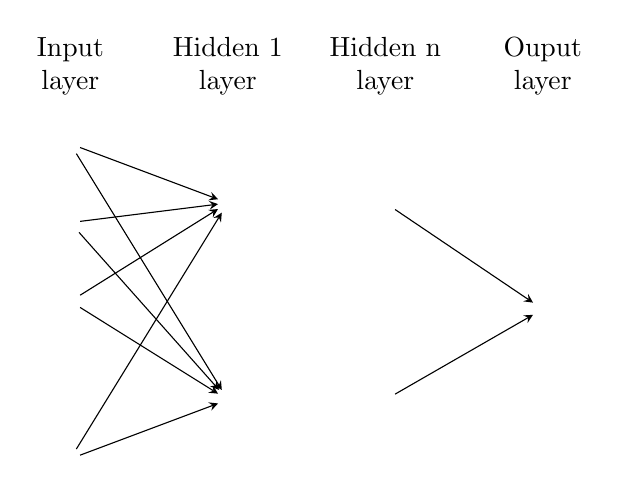
\begin{tikzpicture}[x=1.0cm, y=1.0cm, >=stealth]

\foreach \m [count=\y] in {1,2,3,missing,4}
  \node [every neuron/.try, neuron \m/.try] (input-\m) at (0,2.5-\y) {};

\foreach \m [count=\y] in {1,missing,2}
  \node [every neuron/.try, neuron \m/.try ] (hidden1-\m) at (2,2-\y*1.25) {};

\foreach \m [count=\y] in {missing2,missing2,missing2}
  \node [every neuron/.try, neuron \m/.try ] (hidden11-\m) at (3,2-\y*1.25) {};
  
\foreach \m [count=\y] in {1,missing,2}
  \node [every neuron/.try, neuron \m/.try ] (hidden2-\m) at (4,2-\y*1.25) {};

\foreach \m [count=\y] in {1}
  \node [every neuron/.try, neuron \m/.try ] (output-\m) at (6,0.4-\y) {};


%\foreach \l [count=\i] in {1,2,3,n}
%  \draw [<-] (input-\i) -- ++(-1,0) % (punta de la flecha)
  %  node [above, midway] {$I_\l$};

%\foreach \l [count=\i] in {1,n}
  %\node [above] at (hidden1-\i.north) {$H_\l$};

%\foreach \l [count=\i] in {1,n}
  %\node [above] at (hidden2-\i.north) {$H_\l$};
  
%\foreach \l [count=\i] in {1,n}
 % \draw [->] (output-\i) -- ++(1,0)
  %  node [above, midway] {$O_\l$};

\foreach \i in {1,...,4}
  \foreach \j in {1,...,2}
    \draw [->] (input-\i) -- (hidden1-\j);

\foreach \i in {1,...,2}
  \foreach \j in {1}
    \draw [->] (hidden2-\i) -- (output-\j);

\foreach \l [count=\x from 0] in {Input, Hidden 1, Hidden n, Ouput}
  \node [align=center, above] at (\x*2,2) {\l \\ layer};

\end{tikzpicture}
\caption{Artificial Neural Network Diagram}
\label{fig6}
\end{figure}

The nodes of the input layer are joined to the nodes of the hidden layers, by the multiplication of an attribute by a value $w$ which represents the weight of this attribute in that node. In each node of the hidden layer, there will be a transformation process that creates a new representation of the input data. The same process is repeated subsequently until arriving at the output layer that only consists of a regular linear regression applied to the transformed data. This process for a single node can be seen in Fig.~\ref{fig7}.

\begin{figure}[htbp]
\tikzset{%
  every neuron/.style={
    circle,
    draw,
    minimum size=0.5cm
  },
  neuron missing/.style={
    draw=none, 
    scale=2,
    text height=0.333cm,
    execute at begin node=\color{black}$\vdots$
  },
}

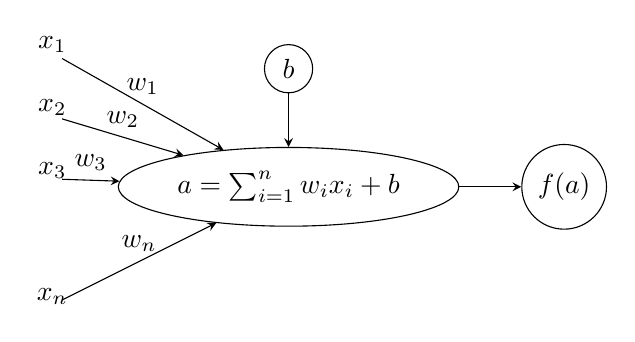
\begin{tikzpicture}[x=1.0cm, y=1.0cm, >=stealth]

\foreach \m [count=\y] in {1,2,3,missing,4}
  \node [every neuron/.try, neuron \m/.try] (input-\m) at (0,2.5-\y*0.8) {};

%\node [draw, ellipse, thick, dash dot, rotate=30, minimum width=7cm, minimum height=5cm, align=center] at   (2,0) {};

\node (hidden1-fun) [draw, ellipse, rotate=0, minimum width=2.5cm, minimum height=1cm, align=center] at   (3,0) {$a = \sum_{i=1}^{n} w_i x_i + b$};

%\node [draw, circle, thick, blue, fill=blue!20, minimum size=2cm, align=center] at   (6,0)   {Data\\\\};

\node (output-1) [draw, circle, minimum size=0.7cm, align=center] at   (6.5,0)   {$f(a)$};

\node (bias-1) [draw, circle, minimum size=0.5cm, align=center] at   (3,1.5)   {$b$};
  
%\foreach \l [count=\i] in {1,2,3,n}
%  \draw [<-] (input-\i) -- ++(-1,0) % (punta de la flecha)
  %  node [above, midway] {$I_\l$};

\foreach \l [count=\i] in {1,2,3,n}
  \node [above] at (input-\i.south) {$x_\l$};


%\foreach \l [count=\i] in {1,n}
  %\node [above] at (hidden2-\i.north) {$H_\l$};
  
%\foreach \l [count=\i] in {1,n}
 % \draw [->] (output-\i) -- ++(1,0)
  %  node [above, midway] {$O_\l$};

\foreach \l [count=\i] in {1,2,3,n}
    \draw [->] (input-\i) -- (hidden1-fun) node[midway,above,rotate=0] {$w_\l$};;

  \foreach \j in {1}
    \draw [->] (hidden1-fun) -- (output-\j);

\draw [->] (bias-1) -- (hidden1-fun);

\end{tikzpicture}
\caption{Transformation process for a single node}
\label{fig7}
\end{figure}

\subsubsection{Training and Validation}

The set of the clear-cutting registers is divided into subsets. For each of the $k$ iterations, the model is validated by subset, $k$ and trained with the remaining $k-1$ subsets, thus, $K$ performance measures are obtained from which their average and standard deviation are computed. 

\paragraph*{a) Performance Metrics} 

The performance measures used are the \textit{Mean Squared Error} (MSE) as in Eq. \eqref{eq2}, the \textit{Root of the MSE} (RMSE) as in Eq. \eqref{eq3}, the \textit{Absolute Mean Error} (MAE) in Eq. \eqref{eq4}, and the Coefficient of Determination ($r^2$) in Eq. \eqref{eq5}. However, the MSE was analyzed as primary metric.

\begin{equation}
\label{eq2}
MSE = \dfrac{1}{m} \sum_{i=1}^{m} ( h(\boldsymbol{x}^{(i)})- y^{(i)})^{2}
\end{equation}

\begin{equation}
\label{eq3}
RMSE = \sqrt{MSE}
\end{equation}

\begin{equation}
\label{eq4}
MSE = \dfrac{1}{m} \sum_{i=1}^{m} | h(\boldsymbol{x}^{(i)})- y^{(i)} |
\end{equation}

\begin{equation}
\label{eq5}
r^{2} = \dfrac
{\sum_{i=1}^{m} ( h(\boldsymbol{x}^{(i)})- \bar{y})^{2}}
{\sum_{i=1}^{m} ( y^{(i)}- \bar{y})^{2}}
\end{equation}

Where $m$ corresponds to the number of samples in the dataset, $\boldsymbol{x}^{(i)}$ is the $i$th sample vector with $n$ sample attributes, $h(\boldsymbol{x}^{(i)})$ the predicted value for the $i$th sample, $y^{(i)}$ is the actual value of the $i$th sample and $\bar{y}$ is the average of the $y$ samples. The depend variable corresponds to the clear-cutting.

\paragraph*{b) Hyperparameters} 

The hyperparameters used for the ANN are as follows:

\begin{itemize}

\item{Number of layers:}
It corresponds to the number of hidden layers in the neural network.

\item{Number of nodes:} 
It corresponds to the number of nodes per hidden layer in the neural network.

\item{Activation function:}
It is a differentiable function that transforms the inputs of a neural network node into an output. 

\item{$\mathrm{K}$:}
It is the number of subsets in which the training set will be validated.

\item{Epochs:}
Corresponds to each of the inputs of the entire training set to be optimized in the neural network. For each validation subset, training must be performed with the rest of the data. For each of these rounds, a certain number of times called epoch is iterated. As the training set is divided into mini-batch and for each mini-batch, an optimization of the model weights is done, then for each epoch several parameter optimizations are made equal to the amount of data in the training set divided by the size of the mini-batch.

\item{Mini-batch:}
Corresponds to the size of the dataset to which the optimization algorithm is applied. That is, the number of samples for which the weighting vector $\boldsymbol{w}$ is optimized.

\item{Learning rate:}
It is one of the most important hyperparameters. This value scaler the gradient in the gradient descent approach, providing the ability to control the step size to be taken when updating the ML parameters.

\end{itemize}

\paragraph*{c) Optimization approach} 

The Adam Optimization Algorithm method is used in Mini-Batches. This approach gradually modifies the model parameters to reduce the MSE. This algorithm corresponds to a variation of the stochastic descending gradient, where the learning rate is varied to control how fast the learning rate is decaying, and how long the gradient can remember from previous step. Also, the L1 regularization technique is applied to control for overfitting during the weight training process.

\paragraph*{d) Experimental Design} 

An exhaustive grid search is done to select suitable hyperparameters.
The candidate hyperparameters are shown in Table~\ref{table3}.


\begin{table}[!t]
\renewcommand{\arraystretch}{1.3}
\caption{Data for the artificial neural network hyperparameters optimization}
\label{table3}
\centering
\begin{tabular}{c || c || c || c || c}
\hline
\bfseries Nª of hidden & \bfseries Nº of nodes & \bfseries Activation & \bfseries Epochs & \bfseries Learning \\
\bfseries layers & \bfseries & \bfseries function &  & \bfseries rates \\

\hline\hline

1	&	25	&	ReLU		&	400	&	0.001 \\
2 	& 	50 	&	Leaky ReLU	&	800	&	0.0001 \\
4 	& 	100 	&	Tanh			&	1600	&	0.00001 \\
6 	&	200	&	Sigmoide		&	 	&	0.000001 \\

\hline
\end{tabular}
\end{table}

The number of models to be tested is $4\times4\times4\times3\times4$ resulting in 768 models. For the remaining hyperparameters described before, the mini-batch was set at 4,096 samples, and the number of folds of the dataset was set at 5.

A grid is also designed to train the LR, with hyperparameters presented in Table~\ref{table4}.

\begin{table}[!t]
\renewcommand{\arraystretch}{1.3}
\caption{Data for gradient descendent linear regression}
\label{table4}
\centering
\begin{tabular}{c || c || c || c }
\hline
\bfseries Epochs 	& \bfseries Learning & \bfseries Minibatch & \bfseries k  	\\
\bfseries  			& \bfseries  rates 	& \bfseries 		& \bfseries        \\

\hline\hline

800		&	0.1		&	2048		&	5	\\
1600		&	0.01		&	4096		&	10	\\
3200		&	0.001	&			&		\\							
6400		&	0.0001	&			&		\\


\hline
\end{tabular}
\end{table}


\paragraph*{e) Selection Criteria} 

The three models with lower average MSE in the validation sets are selected. 

\subsection{Unsupervised visualization model}

\subsubsection{\textit{Self-Organizing Maps} (SOMs)} They are ANNs that allows the visualization of multidimensional data. They can be thought as the non-linear version of principal components. A structure and number of map nodes must be defined, there by the structures studied are 2-dimensional, toroidal and 3-dimensional.


\begin{comment}
In the 2-dimensional structure the nodes are arranged rectangularly. Even though this disposition is widely used, its main drawback is that nodes at the border will have less choices of updating their weights than those that are closer to the center of the structure when the \textit{Best Matching Unit} (BMU) is computed.
\end{comment}

In the 2-dimensional structure the nodes are distributed in a rectangular shape. This disposition is widely used, however, its main drawback is that nodes at the border will have a smaller neighborhood than those that are closer to the center of the structure when the \textit{Best Matching Unit} (BMU) is computed.

The neighborhood is different in the 3-dimensional structure. There is no longer a circular area, instead we have to compute the volume of a sphere. In this 3-dimensional structure, a node has more immediate neighbors than in the 2-dimensional. However, the nodes on the edges have no neighbors beyond the orthohedron structure.

The toroidal structure is an extension of the 2-dimensional structure. The border nodes of the 2-dimensional structure are connected together forming a toroid shape. This structure has the advantage that any BMU has the same number of nodes in its neighborhood.

\paragraph{Algorithm}
The SOM algorithm consists of the steps below.

\paragraph*{a) Initialization} 

The weights of the nodes are initialized randomly using a normal distribution with mean 0 and standard deviation 1. The learning rate $\alpha$ and the neighborhood radius $\sigma$ are initialized.

\paragraph*{b) Selection} 

Randomly select an input vector $\boldsymbol{x}$ from the dataset and pass it through the network.

\paragraph*{c) Find the BMU} 

The node $j$, whose weights $\boldsymbol{w}_j$ are the closest to the vector $\boldsymbol{x}$ based on the euclidean distance measure is chosen as a BMU. Then, the $\boldsymbol{w}_j$ weights are updated by a procedure that makes them closer to the input vector $\boldsymbol{x}$, increasing the likelihood of obtaining similar input vectors in subsequent iterations.

In \eqref{eq6} you can view the process to get the $BMU$.

\begin{equation}
\label{eq6}
BMU(\boldsymbol{x}) = \operatorname*{argmin}_j ||\boldsymbol{x} - \boldsymbol{w}_j || 
\end{equation}
%\quad j=1,\ldots,n

\paragraph*{d) Calculate BMU neighborhood} 

You get the neighborhood radius from the BMU. The nodes within this radius are considered to be in the BMU neighborhood. The objective is to modify the weighting vector $\boldsymbol{w_j}$ of the BMU and the neighboring nodes. The size of the neighborhood is reduced with each iteration. The radius usually starts as the radius of the structure and decreases with the number of iterations.

The radius is computed with the neighborhood function in \eqref{eq7}.

\begin{equation}
\label{eq7}
\theta_{j,BMU(\boldsymbol{x})}(t) = e ^ { -\dfrac
{||\boldsymbol{w}_j - \boldsymbol{w}_{BMU(\boldsymbol{x})}||^{2}}
{2 \sigma (t)}
}
\end{equation}

Where,

\begin{equation}
\label{eq8}
\sigma (t) = \sigma_{initial} \bigg(1 - \dfrac {t} {total\_iterations} \bigg)
\end{equation}

\paragraph*{e) Updating weights} 

The weights of the SOM nodes are constantly updating through the $BMU$ and the nodes in the $BMU$, neighborhood adjust their weights according to the values in the input vector $\boldsymbol{x}$. Moreover, nodes close to $BMU$ update their weights more significantly than nodes far from it. Finally, the weights are updated using Eq.\eqref{eq9}.

\begin{equation}
\label{eq9}
\boldsymbol{w}_j(t+1) = \boldsymbol{w}_j(t) + \eta(t) \theta_{j,BMU(\boldsymbol{x})}(t)(\boldsymbol{x}-\boldsymbol{w}_j(t))
\end{equation}

Where,

\begin{equation}
\label{eq10}
\eta (t) = \eta_{initial} \bigg(1 - \dfrac {t} {total\_iterations} \bigg)
\end{equation}

It is the function of decreasing learning rate, that starts at $\alpha$ and ends at a value close to $0$.

\paragraph*{f) Repeat} 

While there is still remaining iterations, the process will go to step b), otherwise it will return the SOM vector.

\paragraph{Quality measures} 
They are necessary for the selection of the best model and in this work we focus on the followings:

\paragraph*{a) Quantization error (QE)}
Shows how well the nodes weights $\boldsymbol{w_j}$ fit the dataset. It is calculated as the average distance between each of the vectors of the dataset with their respective $BMU$.

\begin{equation}
\label{eq11}
QR = \frac{1}{m} \sum_{i=1}^{m} || \boldsymbol{x}_i -  \boldsymbol{w}_{BMU(\boldsymbol{x}_i)}||
\end{equation}

\paragraph*{b) Topographic error (TE)}
It measures if the SOM preserves the topography of the analyzed data. It is calculated as the proportion of all data vectors for which the first and second $BMU$ are not adjacent. 

\begin{equation}
\label{eq12}
TE = \frac{1}{m} \sum_{i=1}^{m} u(\boldsymbol{x}_i)
\end{equation}

Where,

\begin{itemize}
	\item $u(\boldsymbol{x}_i) = 1$, If the first and second BMU are not adjacent to each other. It measures if the distance between them is greater than $\sqrt{2}$ in the case of 2D and toroidal structures or greater than $\sqrt{3}$ in the case of 3-dimensional structures.
	\item $u(\boldsymbol{x}_i) = 0$, in other cases.
\end{itemize}

The QE is used to select the winning model.

\subsubsection{Clustering}

K-means is an unsupervised classification algorithm that groups data into $k$ clusters based on their similarities. Grouping is achieved by minimizing the distance of each input vector and the centroid of the cluster. The input to the algorithm is the number of clusters and the dataset \cite{some_methods_macqueen}, \cite{k_means_arthur}.

The algorithm consists of 3 steps.

\paragraph*{a) Initialization} 

The number of clusters is defined $k$. The algorithm starts with an initial estimate of $k$ centroids $\boldsymbol{\mu}_j$. These are chosen through $k$ random vectors of the dataset. Each centroid is described by $\boldsymbol{\mu}_j$, where $j = 1,\dots,k$.

\paragraph*{b) Data Assignment} 

Grouping is achieved by minimizing the distance of each sample $\boldsymbol{x}$ to the centroid of the cluster. Each point $\boldsymbol{x}$ of the dataset is assigned to its closest centroid $j$ based on the square of the euclidean distance. 

\begin{equation}
\label{eq13}
\operatorname*{argmin}_{\boldsymbol{\mu}_j} ( {||\boldsymbol{x}-\boldsymbol{\mu}_j||}^{2})
\end{equation}

%\boldsymbol{\mu}_j \in C

\paragraph*{c) Updating} 

The centroid position is updated taking as new centroids the average position of the instances belonging to this group. Let $S_j$ be the set of vectors $\boldsymbol{x}$ assigned to the cluster $j$. The new centroid $\boldsymbol{\mu}_j$ is obtained through \eqref{eq14}.

\begin{equation}
\label{eq14}
\boldsymbol{\mu}_j = \frac{1}{|S_j|} \sum_{\boldsymbol{x}_i \in S_j} \boldsymbol{x}_i
\end{equation}

Steps b) and c) are repeated until the centroids move below a threshold between each step. 
The k-means algorithm guarantees to obtain a result; however, this may be a local optimum. This means that running the algorithm several times and using different starting centroids can give different results.

\paragraph{Quality measures}

\paragraph*{a) Elbow method}
It is a method used to select the number of clusters in the k-means problem \cite{ebk_means_purnima}. The algorithm is run several times for different $k$ and the results are compared. The metric used is the \textit{Sum of the Square Distances} ($SSE$) between the dataset and the centroid of the respective cluster. 

\begin{equation}
\label{eq15}
SSE = \sum_{j=0}^{k} \sum_{ \boldsymbol{x}_i \in S_j} {|| \boldsymbol{x}_i  - \boldsymbol{\mu}_j||}^{2}
\end{equation}

If $k$ increases, this metric is always smaller, reaching the value of zero when $k$ is equal to the number of samples in the dataset. Therefore, an additional strategy must be used. The metric is plotted as a function of $k$ and the selected value is where the rate of decrease is the highest.

\paragraph*{b) Silhouette analysis} 

It corresponds to another method to select the number of clusters \cite{silhouettes_a_rousseeuw}. The following procedure shows how the silhouette coefficient is calculated for a $p_i$ point belonging to a cluster:

\begin{itemize}

\item{Step 1:}
The average distance of $p_i$ is calculated to each of the members of the cluster to which it belongs. This value is called $a_i$.

\item{Step 2:}
For each cluster where $p_i$ is not contained, the average distance of $p_i$ to each of the members of the cluster is calculated.  The lowest average distance corresponds to $b_i$.
	
\item{Step 3:}
The silhouette coefficient for the point $p_i$ is given by \eqref{eq16}.

\end{itemize}

\begin{equation}
\label{eq16}
s_i = \frac{b_i - a_i} { \max(a_i,b_i)}
\end{equation}
The value of $s_i$ is in the range of $[-1,1]$. A positive value indicates that the average distance of $p_i$ to the cluster to which it belongs is less than the average distance to the nearest cluster. While a negative value indicates that the average distance of $p_i$ to the nearest cluster is less than the cluster to which it belongs. Therefore, we want $s_i$ to be positive and $a_i$ as close to zero as possible. 

Finally, the average silhouette coefficient of all points belonging to the problem is calculated for different quantities of clusters. The number of clusters selected is the one with the lowest average.  

\section{Results}

\subsection{Supervised predictive models}

The 64 LR models and the 768 ANN models were solved following the steps presented on the methodology. The best 3 are selected according to the selection criteria corresponding to the MSE. The most important characteristics are obtained for later analysis. Averages and standard deviations are computed from the MSE, RMSE, MAE, and coefficient of determination. Additionally, the time of solution of each model is registered. Tables~\ref{table5} and~\ref{table6} present these results in detail.

\begin{table}[!ht]
\renewcommand{\arraystretch}{1.3}
\caption{Summary of the best linear regression models according to MSE}
\label{table5}
\centering
\begin{tabular}{c || c || c || c }
\hline
\bfseries 		 & \bfseries 1st Model 	& \bfseries 2nd Model 	& \bfseries 3rd Model  	\\

\hline\hline

Learning Rate				&	0.1		&	0.1		&	0.1		\\
Epochs					&	6400		&	6400		&	3200		\\
Mini-Batch				&	2048		&	2048		&	2048		\\
Nº of k-folds				&	5		&	10		&	5		\\
MSE $\bar{x}$				&	3979.206  &	3980.617	&	3986.62	\\
MSE	$\sigma$				&	253.607	&	322.466	&	260.02	\\
RMSE $\bar{x}$			&	63.05	&	63.04	&	63.11	\\
RMSE $\sigma$			&	2.03		&	2.53		&	2.07		\\
MAE $\bar{x}$				&	40.59	&	40.568	&	40.596	\\
MAE $\sigma$				&	0.296	&	0.389	&	0.316	\\
$r^{2}$  $\bar{x}$			&	0.644	&	0.643	&	0.642	\\
$r^{2}$ $\sigma$			&	0.015	&	0.017	&	0.015	\\
Time						&	1340.72	&	3178.21	&	701.24	\\

\hline
\end{tabular}
\end{table}


\begin{table}[!t]
\renewcommand{\arraystretch}{1.3}
\caption{Summary of the best neural network models according to MSE}
\label{table6}
\centering
\begin{tabular}{c || c || c || c }
\hline
\bfseries 		 & \bfseries 1st Model 	& \bfseries 2nd Model 	& \bfseries 3rd Model  	\\

\hline\hline


N° of hidden layers     	&     2    &     2     &     2     \\
N° de nodes    	 		&     200    &     200     &     200     \\
Activation function     	&     Sigmoid    &     ReLU     &     ReLU     \\
Epochs     			&     1600    &     1600     &     800     \\
Learning Rate     		&     0.001    &     0.001     &     0.001     \\
MSE $\bar{x}$     		&     2484.56    &     2492.51     &     2503.26     \\
MSE $\sigma$     		&     169.56    &     185.23     &     173.42     \\
RMSE $\bar{x}$     		&     49.82    &     49.89     &     50     \\
RMSE $\sigma$    		&     1.7    &     1.85     &     1.74     \\
MAE $\bar{x}$     		&     32.71    &     32.55     &     32.64     \\
MAE $\sigma$     		&     0.23    &     0.16     &     0.18     \\
$r^{2}$ $\bar{x}$     			&     0.78    &     0.78     &     0.78     \\
$r^{2}$ $\sigma$     			&     0.01    &     0.01     &     0.01     \\
Time (s)     			&     470.4    &     468.31     &     239.94     \\

\hline
\end{tabular}
\end{table}

\begin{table}[!ht]
\renewcommand{\arraystretch}{1.3}
\caption{Summary of the best models according to MSE}
\label{table7}
\centering
\begin{tabular}{c || c || c }
\hline
\bfseries 		 & \bfseries  Best ANN Model		& \bfseries Best LR Model \\

\hline\hline

MSE $\bar{x}$         &    2484.56     &     3979.206     \\
MSE $\sigma$         &    169.56     &     253.607     \\
RMSE $\bar{x}$         &    49.82     &     63.05     \\
RMSE $\sigma$        &    1.7     &     2.03     \\
MAE $\bar{x}$         &    32.71     &     40.59     \\
MAE $\sigma$         &    0.23     &     0.296     \\
$r^{2}$ $\bar{x}$         &    0.78     &     0.644     \\
$r^{2}$ $\sigma$         &    0.01     &     0.015     \\
Tiempo (s)      &    470.4     &     1340.72     \\

\hline
\end{tabular}
\end{table}

Both approaches show notable differences. All $r^2$ values of the LR models show an out-of-sample value of $64\%$ as opposed to the $78\%$ in the ANNs. For all collected values for ANNs, $25\%$ of the configurations are under 3,450.5 MSE, half are under 13,090.9 and $75\%$ are under 34,851.4. Conversely, for the case of LR, $25\%$ of MSE is under 4,114.3 MSE, half is under 4,623.1 and $75\%$ is under 6,293.6, which shows the superiority of the ANN even when the hyperparameter specification is not the best.

\begin{figure}[!htbp]
\centerline{\includegraphics[width=3.3in]{imagenes/msevse_eng.pdf}}
\caption{Graph of MSE in the training and validation set for the 3rd iteration of the cross validation of the best model}
\label{fig9}
\end{figure}

\begin{figure}[!htbp]
\centerline{\includegraphics[width=3in]{imagenes/tensorFlow.pdf}}
\caption{Representation of the selected model via TensorBoard}
\label{fig8}
\end{figure}

Table~\ref{table7} shows a comparison between the best LR and ANN model respectively, and the main differences between them are highlighted. Fig.~\ref{fig9} shows how the loss in the training and validation sets varies according to the epochs, while Fig.~\ref{fig8} shows the selected model graphically in TensorBoard. 

\subsection{Unsupervised visualization model}

Three types of structures (2D, toroidal and 3D) with different number of nodes were trained. The main characteristics of these structures are detailed in Table~\ref{table8}.

\begin{table}[!ht]
\renewcommand{\arraystretch}{1.3}
\caption{SOM Structures Overview}
\label{table8}
\centering
\begin{tabular}{c | c || c | c | c }
\hline
	&	&  \multicolumn{3}{c}{Number of Nodes} \\ 
\hline
	&	&  64 	&	294	&	729	\\ 	
\hline\hline
\multirow{3}{*}{Structure}		& 	2D		&  $8\times8$	&	$14\times21$	&	$27\times27$	\\ 	
				&	Toroidal	&  $8\times8$	&	$14\times21$	&	$27\times27$	\\ 
				&	3D		&  $4\times4\times4 $		&	$7\times7\times6 $	&	$9\times9\times9 $	\\ 		

\hline
\end{tabular}
\end{table}

Table~\ref{table9} shows the overall results obtained from the different SOMs. The results are presented by structure, the number of iterations, QE, TE, and time. A learning rate of 0.05 is considered to train the neural network.

\begin{table}[!t]
\renewcommand{\arraystretch}{1.3}
\caption{Summary SOM Structures}
\label{table9}
\centering
\begin{tabular}{c || c | c | c | c | c | c}
\hline
\multicolumn{7}{c}{2D Model Results} \\ 
\hline
 & \multicolumn{2}{c|}{QE} & \multicolumn{2}{c|}{TE} & \multicolumn{2}{c}{Time (s)} \\ 
\hline
\hline

Iterations & 500 & 1500 & 500 & 1500 & 500 & 1500 \\ 
8x8 & 0.929 & 0.94 & 0.152 & 0.175 & 2314.083 & 6888.93 \\ 
14x21 & 0.61 & 0.492 & 0.048 & 0.077 & 2399.987 & 7256.778 \\ 
27x27 & 0.494 & 0.374 & 0.024 & 0.035 & 2474.871 & 7538.313 \\ 

\hline

\multicolumn{7}{c}{Toroidal Model Results} \\ 
\hline
 & \multicolumn{2}{c|}{QE} & \multicolumn{2}{c|}{TE} & \multicolumn{2}{c}{Time (s)} \\ 
\hline
\hline

Iterations & 500 & 1500 & 500 & 1500 & 500 & 1500 \\ 	
8x8 & 0.984 & 0.928 & 0.175 & 0.133 & 1827.154 & 5578.438 \\ 	
14x21 & 0.645 & 0.555 & 0.063 & 0.068 & 1824.507 & 5688.549 \\ 	
27x27 & 0.505 & 0.375 & 0.017 & 0.045 & 1841.655 & 5550.733 \\ 	

\multicolumn{7}{c}{3D Model Results} \\ 
\hline
 & \multicolumn{2}{c|}{QE} & \multicolumn{2}{c|}{TE} & \multicolumn{2}{c}{Tiempo (s)} \\ 
\hline
\hline

Iterations & 500 & 1500 & 500 & 1500 & 500 & 1500 \\ 
4x4x4 & 0.99 & 1.01 & 0.166 & 0.15 & 2289.232 & 7041.367 \\ 
7x7x6 & 0.541 & 0.525 & 0.056 & 0.064 & 2479.334 & 7573.549 \\ 
9x9x9 & 0.368 & 0.319 & 0.025 & 0.031 & 2554.009 & 7771.914 \\ 

\end{tabular}
\end{table}

The heat maps for the 729 nodes configuration of each of the different structures can be seen in Figure~\ref{fig10}, Figure~\ref{fig11}, and Figure~\ref{fig12}. Then, using the elbow method and silhouette coefficient, the proper number of clusters were obtained. Figure~\ref{fig13} shows the elbow method in the 3D structure while, 
Figure~\ref{fig14} depicts the silhouette coefficient.

\begin{figure}[htbp]
\centerline{\includegraphics{imagenes/lector2d3.pdf}}
\caption{Heat map for each attribute in the 2D structure with a grid of $27\times27$.}
\label{fig10}
\end{figure}

\begin{figure}[htbp]
\centerline{\includegraphics{imagenes/lectorToroidal2.pdf}}
\caption{Heat map for each attribute in the toroidal structure with a grid of $27\times27$.}
\label{fig11}
\end{figure}

\begin{figure}[htbp]
\centerline{\includegraphics{imagenes/lector3d2.pdf}}
\caption{Heat map for each attribute in the 3D structure with a grid of $9times9times9$.}
\label{fig12}
\end{figure}

\begin{figure}[htbp]
\centerline{\includegraphics{imagenes/elbow_method_eng.pdf}}
\caption{Elbow Method applied to SOM 3D of 729 nodes and 1500 iterations.}
\label{fig13}
\end{figure}

\begin{figure}[htbp]
\centerline{\includegraphics{imagenes/compaSiluet.pdf}}
\caption{Silhoutte Coefficient for the 3 structures with 729 nodes.}
\label{fig14}
\end{figure}

The Figures~\ref{fig15},~\ref{fig16}, and~\ref{fig19} show the clusters obtained using the elbow method. There is a clear separation between clusters except for some nodes, which is explained by the implicit variability of the data. Figures~\ref{fig16} and~\ref{fig18} show a 2-dimensional adaptation of the toroidal and 3D structures, respectively. 

The model with lowest QE corresponds to the 3D configuration of $9\times9\times9$ training with 1500 iterations. A summary of the results is shown in Table~\ref{table9} of the Annex. In the case of numerical variables, the average is used as a reference, while  is used for categorical variables. The thinning variable is called vol\_NOC. Below is a brief summary of each cluster.

\begin{figure}[htbp]
\centerline{\includegraphics{imagenes/kmeans2d.pdf}}
\caption{The 5 clusters obtained in the 2D structure of 729 nodes and 1500 iterations.}
\label{fig15}
\end{figure}

\begin{figure}[!htb]
\begin{minipage}{0.1\textwidth}
\centering
\includegraphics[width=2.5\linewidth]{imagenes/kmeansToroidal2d.pdf}
\end{minipage}\hfill
\begin{minipage}{0.25\textwidth}
\centering
\includegraphics[width=1.2\linewidth]{imagenes/kmeansToroidal2.pdf}
\end{minipage}
\caption{
On the left, the 5 clusters obtained in the toroidal structure of 729 nodes and 1500 iterations. Seen through a 2D structure. On the right, the 5 clusters obtained in the toroidal structure of 729 nodes and 1500 iterations.}
\label{fig16}
\end{figure}

\begin{figure}[!htbp]
\centerline{\includegraphics[width=3in]{imagenes/kmeans3d.pdf}}
\caption{The 3 clusters obtained in the 3D structure of 729 nodes and 1500 iterations.}
\label{fig19}
\end{figure}

\begin{figure}[!htb]
\begin{minipage}{0.1\textwidth}
\centering
\includegraphics[width=4.0\linewidth]{imagenes/kmeansPlano3d.pdf}
\end{minipage}\hfill
\begin{minipage}{0.1\textwidth}
\centering
\includegraphics[width=0.9\linewidth]{imagenes/kmeansLargo3d.pdf}
\end{minipage}
\caption{The 3 clusters obtained in the 3D structure of 729 nodes and 1500 iterations. Seen through a 2D structure of $27\times27$ on the left and $81\times9$ on the right.}
\label{fig18}
\end{figure}


\begin{itemize}

\item{Cluster 1 (Purple):} This cluster is composed of 43.87\% of the data. For all data points slope is an important covariate, since only 300 meters towers were used for thinning. The species are composed of 63.9\% eucalypt (Eucalyptus globulus) and 36.1\% of radiata pine. In this cluster, the most important season is Winter having 71.87\% of the records. The lowest number of workers was obtained in this cluster with an average of 5.53 workers per registry. One forest service company stands out among the four that appear in this cluster, its name is Sinergia Forestal Ariel Guzmán Eirl, which accounts for 45.64\%. 

\item{Cluster 2 (Green):} This cluster has 47.58\% of the data. As in Cluster 1, all operations are done using 300 meters equipment. Additionally, proportion of species is 22.04\% radiata pine and 77.96\% eucalypt. The dominant season of this cluster was Autumn with 48.2\%, although Winter has a 43.84\% of the samples. Even though Sinergia Forestal is also in this cluster, the most representative company is Forestal Mantoverde Ltda. The  Vol\_NOC and effective working time are the lowest of the 3 clusters with 35.16 $m^{3}$ and 5.5 hours, respectively.

\item{Cluster 3 (Red):} This cluster contains 8.55\% of the data. The covariate slope is not important for this cluster, allowing the use of equipment such as cable skidder in 89.79\% and grapple skidder in 10.21\%. The vol\_NOC is the highest of the 3 clusters, doubling the volume in Cluster 1 with 98.44 $m^{3}$. The effective working time and the number of workers were also the highest with 7.51 hours and 7.51 workers respectively. However, unlike the other clusters, the standard deviation of the samples in the cluster is the highest. In this cluster, other forest service enterprises, not seen in the  previous clusters, agglutinate most of the services, being Agricola y Forestal del Sur Ltda the most important with 65.53\% of the data.

\end{itemize}

\section{Discussion}

\subsection{Prediction model}

LR models have higher MSE compared to Neural Networks, showing the latter better adaptation to attributes than linear regression. This is due to their intrinsic complexity that allows them to make more complex data transformations, which make them more adaptable.

The results align with what has been seen in the literature. In \cite{application_of_bhering} and \cite{artificial_neural_kaul}, an improvement is shown between the coefficients of determination of the ANNs with respect to the LR's.  In \cite{artificial_neural_kaul}, a coefficient of determination similar to the one obtained in this investigation was presented, to the problem of estimating the crop yield of corn and soybean. However, in our work a longer difference was obtained when comparing both algorithms.

The MSE shows differences between the training set and the validation set, as shown in Figure~\ref{fig9}. This difference is expected since the validation set is not observable to the algorithm during its training phase.

However, our results are limited by the hyperparameters defined in the Tables \ref{table3} and \ref{table4}, and there is chance they could be improved by performing more tests covering a larger combination of hyperparameters. Thereby, more computational power is required to test more models configurations that arise of increasing the number of hyperparameters, especially in ANN models. 

\subsection{Visualization model}

An improvement in QE was generally obtained as iterations progressed. It became more noticeable as more nodes were added to the structures. The model with lowest QE corresponds to the 3D model of $9\times9\times9$ for 1500 iterations, thus, the main analysis was done based on this model.

The TE tended to increase with the number of iterations, while QE, showed the opposite effect. This may be due to the variability of the data, making more complex for the algorithm to determine the overall position of the BMU of a specific sample. The models with best TE were the toroidal structure with 500 iterations, and the 3D for 1500 iterations, both configured with 729 nodes.

Even though there are nodes with unassigned samples, the average number of assignments per node is 3.8, while the standard deviation is 5.6 in the case of the 3D structure, 5.3 in the toroidal structure, and 5.0 in the 2D model. However, due to the neighborhood function, the empty nodes' weights are still modified by the nearby nodes with assigned samples.

The three structures have similar heat maps. Although they have different geometric structures, in all of them, there are areas with close characteristics in proportion, size, and weight values. For example, the attribute of the number of workers (n\_workers) in the three structures are dominated by green colors, with small red and purple zones.

The correlation can be observed directly from the heat maps. The vol\_NOC has a correlation of 0.56 with the effective working time (effective\_t); this can be seen on all three maps, observing specific zones in the individual maps in Figures~\ref{fig10},~\ref{fig11} and~\ref{fig12}. Generally, when one of these attributes is high, the other is also high. Additionally, there is a negative correlation of -0.3 between the vol\_NOC and terrain slope. This makes clear that in areas where slope is low, the vol\_NOC is higher. Another finding to highlight is that the attribute m3\_ha has a high correlation with density variable (dens), which is observed in map zones where both are similar. Moreover, it can be observed that the Radiata Pine and the Euca Nitens are the most pruned species, while the Euca Globolus, found on sloped terrain, is the least pruned.

The two methods for obtaining the clusters gave different results. The elbow method, in the 2D and toroidal models, gave five different clusters, while for the 3D model, only three (Fig.~\ref{fig15} -~\ref{fig19}). Using the silhouette coefficient, two clusters were obtained in all structures (Fig.~\ref{fig14}). Subsequent analyses are made with the 3 clusters obtained from the 3D model with 729 nodes, because it obtained the best QE value.

A $27\times27$ display of the three structures is shown in the Figures ~\ref{fig15},~\ref{fig16} and~\ref{fig18}. If we compare the results given by 2D and toroidal models, their main clusters have similar counting of nodes, with 310 and 315 nodes, followed by 264 and 266 nodes respectively. The remaining clusters have greater variability, and they were not compared with the 3D structure.

The highest vol\_NOC is obtained when there is no slope. It can be inferred that this value was higher because it is easier to reach a terrain in which there is no slope. In sloped terrain, the use of specialized machinery such as the 300 m tower is consistently selected by the model. The predominant season for thinning is Winter. Conversely, the Spring and Summer seasons have low number of samples in each clusters, being null the data in summer for Cluster 2.

Also, there are limitations on the selection of parameters, because there are numerous combinations that could have been tested. The number of nodes is variable, and depending on the structure of the map, this will delivers different results. Moreover, the number of iterations is an influential factor in the performance measures.

To the best of our knowledge SOMs have not been used in thinning processes in the literature, and the analyses and comparisons made in this work present the most commonly used performance measures available in literature. Additionally, 3D structures have been rarely used because the inherent difficulty of its visualization.

\section{Conclusions}

This study shows the efficacy of using supervised and unsupervised neural networks to study clear-cutting and thinning operations, respectively. Since the use of ML techniques applied to thinning and clear-cutting operations it is possible to perform a better analysis of forest activities and predict the operational efficiency of service companies. First, the multilayer perceptron artificial neural network is use to predict clear-cutting achieved by contractors in farms located in the surroundings of the Bío-Bío and Maule regions, Chile. Second, we use SOMs for the analysis of the thinnings processes, in farms located in the same area.

The proposed neural network obtains an out-of-sample MSE and $r^{2}$ of 2189.91 and 0.78 respectively, versus the 3725.11 and 0.64 from a linear regression. The results suggest that using an ANN to make predictions is an important improvement for this kind of operations in the forestry sector.

The use of SOMs coupled with the k-means algorithm for clustering is a powerful analysis tool. It is possible to rearrange complex information in a lower dimensional projection to recognize patterns that otherwise would be difficult visualize with the naked eye. The use of 3D SOMs demonstrated to outperform the classics 2D and toroidal configurations, which is also another contribution of this study.

Future work for the ANN used in clear-cutting prediction could include the testing of new configurations of hyperparameters, or the testing of other ML methods such as Random Forest or Boosted Trees which have shown promising results in other fields. In regard to SOMs, the analysis can be complemented with the addition of more attributes, such as, information about the climate, topographic characteristics, characteristics species or others, allowing a deeper analysis of the thinning problem to find even more insightful patterns. 

\bibliographystyle{IEEEtran}
\bibliography{biblio_paper}

\onecolumn
\appendix 

\begin{table}[htpb]
\renewcommand{\arraystretch}{1.3}
\caption{Descriptive summary of variables studied, at cluster level for the 3D structure of $9\times9\times9$ nodes.}
\label{table10}

\centering

\begin{tabular}{l || c c c}

& \multicolumn{3}{c}{Clusters} \\ 
& 1 $(n = 1205)$	& 2 $(n = 1307)$	& 3 $(n = 235)$ \\

\hline
\hline

Numerical Variables  $(\bar{X}\pm D.E.)$ \\
\\
Density & 7.14 (0.25) & 7.05 (0.42) & 6.98 (0.33) \\ 
$M^3$ of trees & 0.52 (0.11) & 0.45 (0.05) & 0.54 (0.21) \\ 
$M^3$ of trees per hectare & 18.17 (3.59) & 15.88 (3.3) & 16.43 (3.71) \\ 
Number of workers & 5.53 (1.58) & 6.45 (0.66) & 7.51 (3) \\ 
Effective work time & 5.68 (1.57) & 5.5 (1.79) & 7.51 (2.48) \\ 
Land x-coordinate & 650780.75 (14828.88) & 668975.7 (4365.02) & 656593.9 (13127.5) \\ 
Land y-coordinate & 5858754.09 (18024.36) & 5889334.35 (7857.49) & 5870099.52 (14531.77) \\ 
Thinning & 40.88 (20.88) & 35.16 (18.02) & 98.44 (136.56) \\ 
\\
Slope (Frequency (\%)) &  &  &  \\ 
Yes & 1205 (100\%) & 1307 (100\%) & 0 (0\%) \\ 
No & 0 (0\%) & 0 (0\%) & 235 (100\%) \\ 
\\
Specie (Frequency (\%)) &  &  &  \\ 
Euca Globulus & 770 (63.9\%) & 288 (22.04\%) & 33 (14.04\%) \\ 
Eucs Nitens & 0 (0\%) & 0 (0\%) & 24 (10.21\%) \\ 
Pino Radiata & 435 (36.1\%) & 1019 (77.96\%) & 178 (75.74\%) \\ 
\\
Type of equipment (Frequency (\%)) &  &  &  \\ 
Grapple skidder & 0 (0\%) & 0 (0\%) & 24 (10.21\%) \\ 
Cable skidder & 0 (0\%) & 0 (0\%) & 211 (89.79\%) \\ 
300 meters tower & 1205 (100\%) & 1307 (100\%) & 0 (0\%) \\ 
\\
Season (Frequency (\%)) &  &  &  \\ 
Winter & 866 (71.87\%) & 573 (43.84\%) & 148 (62.98\%) \\ 
Autumn & 159 (13.2\%) & 630 (48.2\%) & 60 (25.53\%) \\ 
Spring & 106 (8.8\%) & 104 (7.96\%) & 11 (4.68\%) \\ 
Summer & 74 (6.14\%) & 0 (0\%) & 16 (6.81\%) \\ 
\\
EMSEFOR (Frequency (\%)) &  &  &  \\ 
Agricola y Forestal del Sur LTDA. & 0 (0\%) & 0 (0\%) & 154 (65.53\%) \\ 
Empresa Marquez y Figueroa LTDA. & 0 (0\%) & 0 (0\%) & 57 (24.26\%) \\ 
Forestal Mantoverde LTDA. & 170 (14.11\%) & 536 (41.01\%) & 0 (0\%) \\ 
Forestal Reloncavi LTDA. & 158 (13.11\%) & 355 (27.16\%) & 0 (0\%) \\ 
Import. y Comer. Metsakone LTDA. & 0 (0\%) & 0 (0\%) & 24 (10.21\%) \\ 
Servicios Forestales J. Gonzalez LTDA. & 213 (17.68\%) & 103 (7.88\%) & 0 (0\%) \\ 
Sinergia Forestal Ariel Guzmán Eirl. & 550 (45.64\%) & 184 (14.08\%) & 0 (0\%) \\ 
Sociedad forestal Fasi LTDA. & 114 (9.46\%) & 129 (9.87\%) & 0 (0\%) \\ 

\end{tabular}
\end{table}


\end{document}
